\chapter{Background}

\section{Introduction}

Majorana bound states (MBS) can be used to store quantum information protected from the local environment.
MBS can be realised in a hybrid quasi-one dimensional system that combines a strong-spin orbit semiconductor with proximity induced superconductivity.
Semiconducting nanowires and two-dimensional electron gases (2DEG) are candidates for creating such devices.

Majorana based quantum computation requires controlled interaction of multiple MBS in a two dimensional device.
The ground state evolves following controlled quantum operations by selectively coupling different MBS pairs.
Nanowires networks or gate-defined networks in 2DEGs have been studied experimentally and theoretically as platforms for Majorana based computation.

While coupling a single MBS pair can be done using a quantum dot, selective coupling of multiple pairs remains a challenge.
On one hand, there are geometrical constraints given by tuning multiple separate nanowires in the topological phase.
On the other hand, the coupling of multiple pairs should be optimised simultaneously by the device geometry.
Therefore, design and operate a multi Majorana device is a non-trivial task.
 
The simplest system where multiple MBS can couple non-trivially is in a trijunction geometry.
In this thesis we propose a semiconducting cavity connected to three Majorana nanowires that allows for an all-electric controlled interaction between all pairs of MBS.

Initially, the role of geometry is investigated by simulating several cavity geometries and extracting the MBS coupling in the strong coupling regime.
We found that the geometrical configuration of the trijunction modulates the coupling of the MBS pairs.
Several cavity geometries are analysed, and a triangular cavity with varying angle is found to have the largest coupling for all pairs simultaneously.

Finally, a realistic model is studied via electrostatic simulations of a gate-defined triangular configuration defined on a 2DEG.
The non-local nature of the gates makes the nanowire positions crucial in order to recover the effects found for the purely geometric case.
The role of each set of gates and the range of voltages used to operate the device are discussed.
The electrostatics effects of the gate-defined triangular cavity are analysed and the operational point is described.


\section{Majorana bound states}

\begin{figure}[h!!]
\centering
  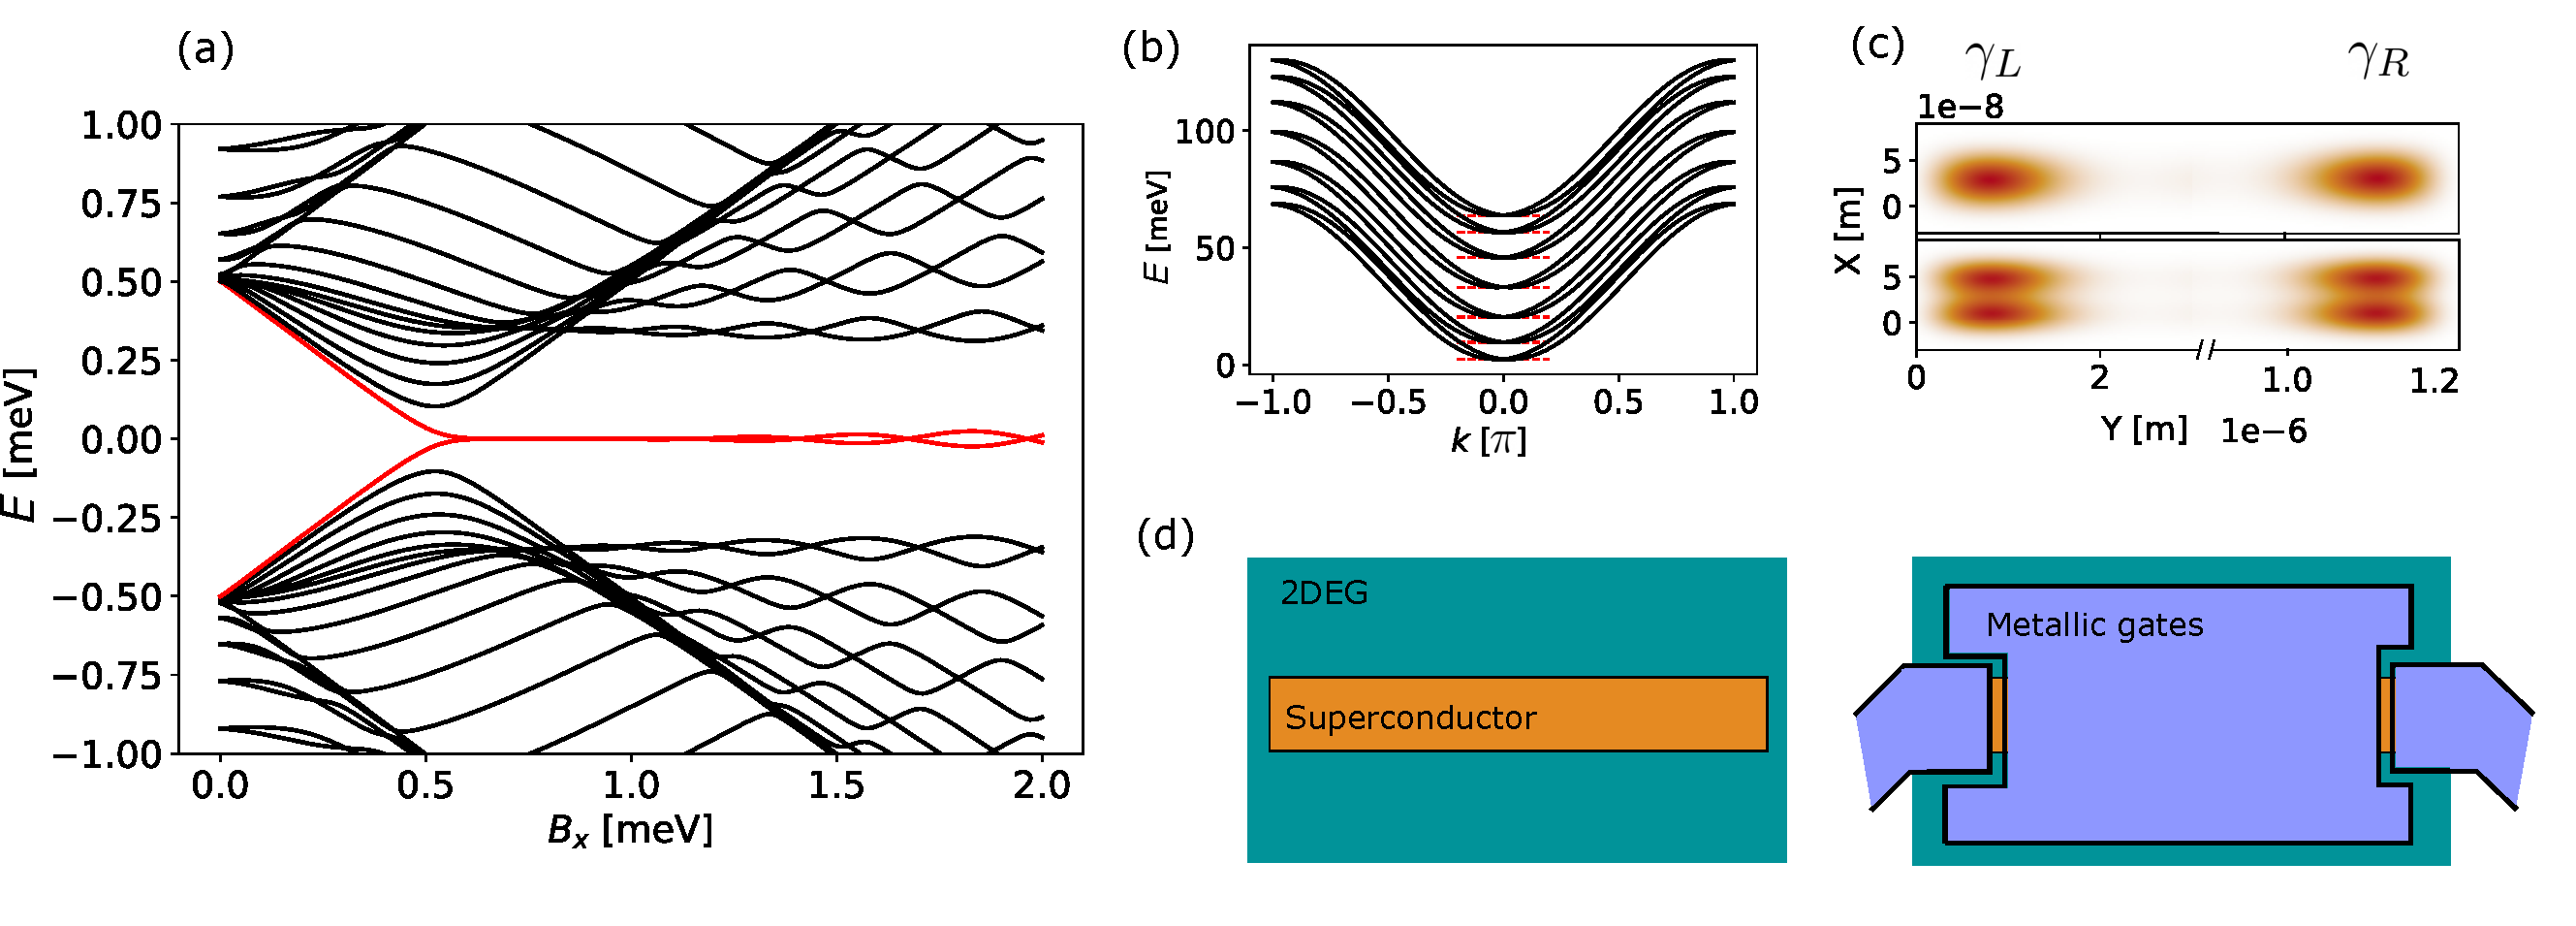
\includegraphics[width=0.95\linewidth]{figures/majorana_intro.pdf}
  \caption{Simulations of a Majorana nanowire as described in Eq. \eqref{eq:ham_maj}. The following parameters will be used in all simulations:  $\Delta=0.5$[meV], $\alpha=0.3$[eV A], and $m^*=0.023 m_e$. Each simulated nanowire has length $L=120*a$ and width $W=7*a$ where $a=10$[nm] is the lattice constant size. (a) Topological phase transition as a function of Zeeman field $B_x$. Lowest mode (red) sticks to zero after crossing the critical field. (b)  Transverse bands along the translational invariant direction with $\Delta=0$. The chemical potential is tuned to the bottom of each band (red dashed lines) to create Majoranas. (c) Majorana wavefunctions for the lowest two bands. (d) Illustration of how a Majorana nanowire is built on a 2DEG. Left panel shows the 2DEG with a superconducting stripe on top. Right panel shows the system after the deposition of the gates.}
  \label{fig:intro}
\end{figure}

MBS populate the non-local degenerate ground state of a topological superconductor\cite{Alicea2011}.
Under the appropriate conditions, a spinless one-dimensional $p$-wave superconductor contains two zero-energy excitations that are exponentially localised at the edges of the system. 
Together, these two zero-energy modes encode a single fermionic mode that can be empty or occupied, 
\begin{equation}
f = \frac{\gamma_{L} + i\gamma_{R}}{\sqrt{2}}, \quad f^{\dagger} = \frac{\gamma_{L} - i \gamma_{R}}{\sqrt{2}},
\end{equation}
where $\gamma_{i} = \gamma_{i}^{\dagger}$ are Majorana operators that satisfy $\{ \gamma_{i}, \gamma_{j} \} = 2\delta_{ij}$.
%The ground state $\ket{\Psi}$ is two-dimensional, and it is spanned by the states $\ket{0}$ and $f^{\dagger}\ket{0}$, i.e. empty and occupied states.

%\textit{Since a pair of spatially separated MBS encode a single fermionic mode, its quantum state is protected against local errors by particle-hole symmetry.}
In a sufficiently long nanowire, MBS are decoupled from each other, and noise sources will interact with each of them individually.
The interaction with a single MBS is proportional to a single Majorana operator, i.e. $\gamma \sim f + f^{\dagger}$, and thus it will change the parity of the system.
In a superconductor, however, electrons can only enter or leave as Cooper pairs, which means that the parity is conserved. 
Therefore, individual MBS are immune to local noise sources.

Consequently, only even powers of Majorana operators are allowed in the Hamiltonian.
The simplest allowed term describes the coupling of a pair of MBS.
In a single nanowire, or in a linear array of them, it is only possible implement this term with successive MBS.
It is given by,
\begin{equation}\label{eq:H_pair}
H_{pair} = i E_{LR} \gamma_{L} \gamma_{R} = E_{LR} (1 - 2 f^{\dagger} f).
\end{equation}
Here, $E_{LR}$ is the tunnelling coupling between the two MBS.
Consequently, a general state within the degenerate subspace evolves as,
\begin{equation}
\ket{\Psi}  = \alpha \ket 0 +\beta \ket 1 \rightarrow U(t) \ket{\Psi} = \alpha \ket 0 + \beta e^{2 i E_{LR} t} \ket 1.
\end{equation}
%\textit{The ground state can only evolve by non-local operations that involve pairs of MBS.}

However, universal quantum computation cannot be built from using only quadratic fermionic terms as in Eq. \ref{eq:H_pair}.
Controlled interaction between MBS from different fermions are essential to Majorana based quantum computation\cite{Sau2011, Leijse2021, Bauer2018}.
Therefore, a higher dimensional structure where multiple MBS converge is required in order to do Majorana computation.
%In the presence of multiple MBS pairs, on the other hand, each parity subspace can be used as a computational subspace.
%\textit{By controlling the coupling between different MBS pairs, one can control the ground state evolution}, that is,

\section{Experimental platforms}

%MBS were only in Kitaev's toy model until several proposals for realising them on solid-state devices appeared.
%The main problem was that electrons are not spinless, and $p$-wave superconductor have not been found so far.
%Superconductors pair electrons with different spins, i.e. singlets, as suggested by BCS theory.
%However, by combining a $s$ wave-superconductor, such as Al, and a material with strong spin orbit coupling, such as $InAs$ or $InSb$, one can effectively realise spinless fermions in the presence of a magnetic field.
%However, creating such material combination 
\textit{MBS can be realised in quasi one-dimensional systems defined on two-dimensional electron gases (2DEGs), or semiconducting nanowires, with strong spin-orbit and in proximity to a superconductor.}
The Hamiltonian that realises a Majorana nanowire\cite{Alicea2011} is,
\begin{equation}\label{eq:ham_maj}
\mathcal{H} = \sum_k \Psi_k^\dagger H(k) \Psi_k  ,\quad H(k) =  \left[ \frac{|\mathbf{k}|^2}{2 m^*} - \mu + \alpha(k_x \sigma_y - k_y \sigma_x) \right] \tau_z + B_x \sigma_x  + \Delta \tau_x.
\end{equation}
Here, $\Psi_k^\dagger = (f_{k\uparrow}^\dagger, f_{k\downarrow}^\dagger, f_{k\uparrow} f_{k\downarrow})^T$ are the Nambu spinors in $k$ space, $\mu$ is the chemical potential, $\mathbf{k}$ is the 2D wave-vector, $\alpha$ is the spin orbit interaction, $B_x$ is the Zeeman field, $\Delta$ is the superconducting gap, and $\sigma$ and $\tau$ are Pauli matrices for the spin and particle-hole basis.
MBS appear as zero energy excitations of this Hamiltonian when $B_x^2 \geq \sqrt{\mu^2 + \Delta^2}$.

\textit{Realising such material combination is a challenge, and MBS transport signatures are not unambiguous\cite{Vuik2019,Liu2018}.}
For example, superconductivity and magnetic fields compete with each other.
On the other hand, MBS signatures can be reproduced by states localised in material defects or impurities.
Consequently, most of the current work in this field is focused on unambiguously finding a single MBS pair.

Truly one-dimensional systems do not exist.
There is a translational invariant direction, and at least one direction with finite width $W$.
The energy of each mode has a contribution from both, and it is given by,
\begin{equation}
E_{n}(k) = \frac{\hbar^{2}}{2m^*} \left( k^{2} + \frac{\pi^{2} n^{2}}{W^{2}} \right).
\end{equation}
Here, $m^{*}$ is the effective mass and the spin orbit splitting is not considered.
Independent MBS with different momentum profiles can be formed at each transverse mode when the chemical potential is at the bottom of the corresponding band\cite{Reeg2018}.

%Multiple channel become relevant in the presence of disorder.
%It couples differently to each momentum sub band, which will induce band mixing as has been suggested in experiments.

%\textit{Disorder in the nanowire bulk can be detrimental for MBS since it affects its localisation and properties, such as induced gap, while disorder inside the superconductor enhances the induced gap in the nanowire.}

\subsection{Two dimensional electron gases}

In order to build a multi Majorana device we require a flexible 2D platform where multiple nanowires can be easily attached.
Furthermore, it been shown that properties of Majorana devices can be modulated by changing the device geometry.
\textit{2DEGs appear as an interesting platform for since arbitrary geometries can be created using electrostatic gates.}
On the other hand, high-quality networks of semiconducting nanowires can be built, but geometries are limited to straight configurations.

\textit{Parallel Majorana nanowires are the basic elements for a complex Majorana device.}
A single nanowire on a 2DEG can be created by adding a superconducting strip on top of the selected region as shown in Fig. \ref{fig:intro} (d).
Then, a top gate is deposited next on top of the device such that depletes the surrounding 2DEG.
A narrow quasi-one dimensional channel is created below the superconductor where the gate electric field is screened\cite{Hell2017}.
Following this procedure, multiple parallel nanowires can be created in a 2DEG by selectively depositing superconducting covers.

\textit{There are several Majorana experiments on 2DEGs that have shown promising evidence for scalable and complex devices.}
Initial experiments\cite{Shabani2015,Kjaergaard2016} focused on characterising the properties of semiconducting layers with a superconducting cover.
Advances in material growth allowed for clean interfaces with a hard superconducting gap to develop into the nanowire region.
Later experiments focused on tunnel spectroscopy of stripe-like geometries\cite{Suominen2017} where a zero bias peak (ZBP) was found.
However, due to disorder and defects such ZBPs have most likely a trivial origin from Andreev states rather than MBS.
Nevertheless, efforts to develop complex devices in 2DEGs are made and new promising materials are being studied.

\subsection{Electrostatic gates}

The potential landscape in a 2DEG can be controlled by deposition of metallic gates on a top layer with an insulating barrier in between that smooths the potential profile\cite{Antipov2018}.
\textit{The electrostatic potential in a 2DEG is found by solving the Poisson equation using a finite elements method on the device geometry.}
The potential landscape, $U(\mathbf{r})$, for a given geometrical configuration can be found by solving Laplace equation,
\begin{equation}\label{eq: laplace}
\nabla \cdot \left[ \varepsilon_r(\mathbf{r}) \nabla U(\mathbf{r}) \right] = 0.
\end{equation}
Here, $\varepsilon_r$ is the relative permittivity of each layer in the material stack.
In general, the quantum electrostatics problem is more complicated due to the interaction of dopant charges with the potential.
However, our problem is simpler since no extra charges are required.

%\textit{Electrostatic effects play a crucial role in designing and operating Majorana devices}.
%Characterisation of Majorana nanowire is done via transport measurements that require tunnel coupled leads and gates.
%Furthermore, gates have a non-local effect on the potential landscape that differs between experimental platforms.
%For example, nanowires have a partial superconducting coating that allows for the electric field to penetrate and control the semiconductor and superconductor weight of the wavefunction.
%In 2DEGs, on the contrary, the superconducting coat fully covers it, which screens electrostatic effects.

\section{Majorana bound states in a trijunction}

In order to create a Majorana qubit, at least three MBS with local pair interactions are required\cite{Alicea2011}.
The device that realises this selective coupling is called a trijunction.
It contains two parts: three nanowires, and a central cavity that mediates the coupling.
In such a system, demonstration of the simplest non-trivial Majorana evolution experiment can be done.

The geometrical configuration of the trijunction is subject to two main constraints:
On one hand, nanowires must be parallel since the topological phase closes for small deviations of the magnetic field.
On the other hand, nanowires must have a significant separation from each other such that MBS are well isolated.
Consequently, the design of a trijunction geometry with selective coupling between MBS pair is a non-trivial task.

Previous trijunction designs\cite{Hell2017} have studied MBS coupling in the tunnelling regime.
The trijunction is defined using gates placed on top of a 2DEG, and it is operated by controlling the voltages of the different gates.
In this context, the MBS coupling relies entirely on wavefunction overlap along the cavity. 
Consequently, MBS pairs acquire relatively small couplings with the advantage of not introducing any extra sub gap state.

On the other hand, in the strong coupling the MBS coupling is mediated by cavity states but with extra levels present inside the gap.
Nevertheless, the coupling energy of the MBS pairs can become significantly larger, i.e. comparable with the induced gap.
The modulation of the coupling now relies on the cavity geometry.
Interestingly, it has been shown that properties Majorana devices can be optimised by using geometrical effects.
In this context, this work explores the geometrical dependence of selectively coupling multiple MBS pairs in a Majorana trijunction.

%\textit{There are two main approaches for MBS quantum computation: braiding and joint parity measurements.}
%Braiding was initially proposed as moving MBS around each other in gate defined nanowire networks. 
%However, this method requires high degree of control and is highly susceptible to thermal errors\cite{Pedrocchi2015}.
%On the other hand, joint parity measurements coupling multiple pairs of MBS by using co-tunnelling processes between different MBS on superconducting islands.


%\textit{However, design and operation of a trijunction are non-trivial tasks.}
%Simultaneous tuning of gate voltages and relative phase difference is required to optimally operate a trijunction.
%Selection of the MBS pair and cavity modes is realised by electrostatic gates controlling the potential on each region.
%Furthermore, relative phase differences between MBS modulates the coupling as in the fractional Josephson effect.
%The phase will be shifted by the presence of complex hopping terms and by the nanowires relative position.

%\begin{enumerate}
%\item The dimension of the computational Hilbert space depends on the number of MBS, and thus multiple parallel Majorana nanowires are required for MBS based quantum computing.
%\item 
%\item An equivalent approach that does not require to move the MBS is given by joint parity measurements\cite{Bonderson2008}, but it requires simultaneous measurement of different pairs of MBS.


%\section{Quantum dot mediated coupling}

%\begin{enumerate}
%\item A single nanowire coupled to a quantum dot (QD) allows to measure the parity of a pair of MBS via a measurement of the charge in the dot.
%\item In a single nanowire model, the interaction is controlled by the overlap of the MBS pair which depends on the wire length.
%\item Two nanowires with a QD in the middle recovers the well-know Josephson junction whose spectra can be controlled by the phase difference between the two superconductors.
%\item The fractional Josephson effect, $4\pi$ phase periodicity, is a consequence of the presence of a zero-energy fermionic mode made of two MBS.

%\end{enumerate}

